\documentclass[11pt]{article}

% Change "review" to "final" to generate the final (sometimes called camera-ready) version.
% Change to "preprint" to generate a non-anonymous version with page numbers.
\usepackage[review]{acl}

% Standard package includes
\usepackage{times}
\usepackage{latexsym}
\usepackage{booktabs}
\usepackage{graphicx}
\usepackage{amsmath}
\usepackage{amssymb}
\usepackage{multirow}
\usepackage{subcaption}
\usepackage{url}
\usepackage{microtype}

\title{Whole Questions or Query Fragments? A Controlled Study of Bengali- and Telugu-to-English Retrieval}

\author{Anonymous ACL submission}

\begin{document}
\maketitle

\begin{abstract}
We study how Bengali and Telugu questions should be represented when searching an English document collection. Using XOR-TyDi and the English Wikipedia DPR corpus, we compare complete questions with machine translations, semantic fragments, random controls, and multi-view rewrites. We test two multilingual retrievers: BGE-M3 and multilingual-E5-small. Under the tested fusion methods, separately encoded semantic fragments perform worse than complete questions. Adding semantic tags also shows no improvement over a length-matched random-word control. English translation improves Bengali retrieval with both models, but provides no measurable benefit for Telugu with BGE-M3. At matched candidate budgets, combining dense, sparse, and late-interaction channels provides little or no coverage improvement, and cross-encoder reranking does not improve final recall. Our results suggest that complete questions are a stronger default than explicit semantic fragments, while the value of translation depends on the language and retriever.
\end{abstract}

\section{Introduction}
\label{sec:intro}

Cross-lingual information retrieval (CLIR) in low-resource language pairs is foundational for non-English question answering and retrieval-augmented generation (RAG) \citep{asai2021xor}. In typical asymmetric settings, an information-seeking user poses a query in a low-resource language (e.g., Bengali or Telugu), while the target knowledge resides within an extensive English collection such as the English Wikipedia DPR corpus containing over 21 million passages \citep{karpukhin2020dense}.

A common hypothesis in recent literature posits that compressing a natural question into a single dense vector incurs substantial representation loss, washing out granular entities, temporal constraints, or relational qualifiers \citep{weller2024when}. Consequently, numerous studies have advocated for \emph{query decomposition} into structured semantic sub-components (entities, relations, constraints), multi-query generation via large language models (LLMs), or pseudo-relevance feedback.

In this work, we ask: \textbf{Where does representation loss actually occur in cross-lingual retrieval, and which interventions genuinely change retrieved evidence?} Rather than evaluating proposed techniques in isolation, we conduct a controlled empirical study on the XOR-TyDi benchmark \citep{asai2021xor} across Bengali ($n=312$) and Telugu ($n=238$) retrieving against the 21M-passage English Wikipedia DPR collection. We structure our investigation around three core research questions:
\begin{itemize}
    \item \textbf{RQ1 (Granularity and Controls):} Do semantic query fragments improve Bengali- and Telugu-to-English retrieval over complete questions, and do they outperform matched segmentation and expansion controls?
    \item \textbf{RQ2 (Translation $\times$ Language $\times$ Retriever):} How does English translation affect Bengali and Telugu retrieval across BGE-M3 and multilingual-E5-small?
    \item \textbf{RQ3 (Channel Diversity and Candidate Budgets):} Under matched candidate budgets, when does heterogeneous retrieval increase answer-bearing candidate coverage, and does cross-encoder reranking preserve that gain under character budgets?
\end{itemize}

Through rigorous matched controls—including random span segmentation and length-matched random word additions—we find that modern bi-encoders perform best when provided complete query context. The tested facet decomposition and fusion methods underperform complete-query retrieval, and we detected no improvement from semantic expansion over a matched random-word control. Furthermore, while multi-channel similarity fusion (dense, sparse, and late interaction) numerically surfaces additional candidate passages under expanded candidate pools, deep cross-encoder rerankers do not consistently promote these rescued passages into tight character budgets.

We will release our complete codebase, prompt revisions, model revision identifiers, runfiles, and evaluation scripts upon acceptance to ensure exact reproduction.

\section{Related Work}
\label{sec:related}

\paragraph{Structured and Faceted CLIR.} Early cross-lingual retrieval addressed translation ambiguity via probabilistic structured queries (PSQ) and bilingual dictionaries \citep{pirkola1998effects,darwish2003probabilistic}. Modern dense retrievers instead project queries and documents into shared semantic embedding spaces \citep{karpukhin2020dense,wang2022multilingual}. To address entity degradation in dense vectors, recent studies propose extracting named entities and relational constraints as independent subqueries \citep{darwish2003probabilistic}. However, prior work rarely benchmarks semantic decompositions against matched random segmentations or length-controlled baselines.

\paragraph{LLM Query Transformation.} Query expansion and multi-query rewriting via instruction-tuned LLMs have become standard components of RAG pipelines \citep{jagerman2023query}. While effective for weak lexical baselines, recent evidence demonstrates that generative query rewriting frequently underperforms intact queries when paired with modern dense encoders \citep{weller2024when}. We evaluate whether semantic structuring or full-sentence multi-view expansions can surpass intact questions under controlled conditions.

\paragraph{Multilingual Encoders and Late Interaction.} Multilingual bi-encoders such as BGE-M3 \citep{chen2024bge} and multilingual-E5 \citep{wang2022multilingual} support diverse similarity modalities, including dense embeddings, sparse lexical heads, and multi-vector ColBERT late interaction \citep{khattab2020colbert,nair2022transferring}. Prior benchmarks typically evaluate these similarity channels independently; here, we evaluate their joint ability to surface and promote candidates through cross-encoder reranking.

\begin{figure}[t]
\centering
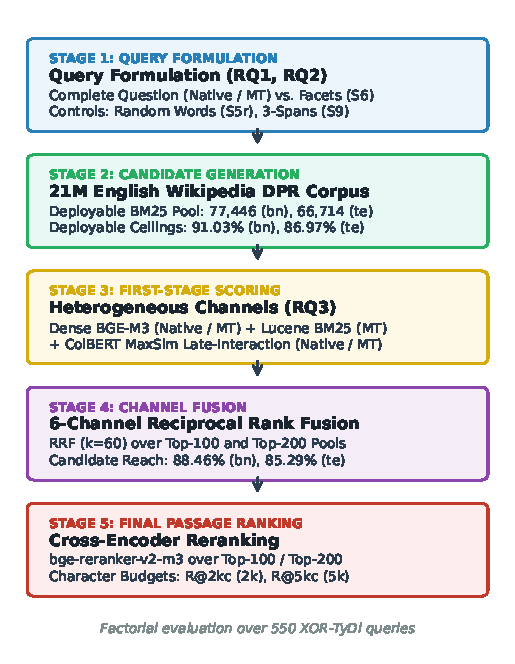
\includegraphics[width=\columnwidth]{fig0_pipeline_portrait.pdf}
\caption{End-to-end evaluation pipeline in single-column portrait layout, depicting query formulation, candidate pooling across 21M Wikipedia passages, heterogeneous channel scoring, RRF fusion, and cross-encoder reranking.}
\label{fig:pipeline_flow}
\end{figure}

\section{Experimental Setup and Protocol}
\label{sec:setup}

\paragraph{Benchmark and Corpus.} We evaluate on the development set of XOR-Retrieve \citep{asai2021xor}, comprising typologically distinct Indic languages: Bengali (\texttt{bn}, $n=312$) and Telugu (\texttt{te}, $n=238$). Queries are evaluated against the 21,015,324-passage English Wikipedia DPR corpus \citep{karpukhin2020dense}.

\paragraph{Relevance Definition.} In XOR-TyDi, passage relevance is evaluated by \emph{answer-string containment}: a retrieved passage is marked relevant if and only if it contains at least one of the gold short answer strings as an exact substring. This character-containment criterion reflects surface text presence rather than graded human semantic relevance.

\paragraph{Evaluation Metrics and Budgets.} We report retrieval recall under fixed character budgets: Recall at 2,000 characters (\textbf{R@2kc}) and 5,000 characters (\textbf{R@5kc}). We emphasize that while the official XOR-TyDi benchmark script \citep{asai2021xor} specifies token accumulation via NLTK word tokenization, our primary evaluations implement a character-budget cutoff ($\approx 3.1$ and $7.7$ passages given average passage lengths of $\approx 645$ characters). We report token-budget metrics in the appendix. We also report candidate coverage (\textbf{R@100} and \textbf{R@200}) and the Catastrophic Failure Rate (\textbf{CFR}), defined as $P(\mathrm{R@100}=0)$.

\paragraph{Candidate Pool Construction and Diagnostic Reference.} Because exhaustive scoring is impractical, we evaluate dense and late-interaction methods by reranking a shared candidate pool generated from full-corpus BM25 searches (up to top-100 passages per variant).
\begin{itemize}
    \item \textbf{Deployable Candidate Pool:} Formed exclusively from native queries, machine translations, and automated decompositions (77,446 passages for Bengali; 66,714 for Telugu). All primary experiments use this deployable pool.
    \item \textbf{Diagnostic Reference Pool:} Additionally incorporates passages retrieved using the human reference translation (S8) solely for diagnostic headroom analysis without test leakage.
\end{itemize}
Table~\ref{tab:pool_stats} reports candidate pool recall ceilings.

\paragraph{Exploratory Development-Set Evaluation.} Because test-set relevance judgments are withheld by benchmark organizers, all evaluated methods, fusion weights, controls, and comparisons are evaluated on the XOR-TyDi development set. In accordance with rigorous methodology, these results are reported as exploratory rather than confirmatory. Holm-Bonferroni adjusted $p$-values provide family-wise error protection across our planned contrasts on this sample rather than out-of-sample confirmatory proof.

\begin{table}[t]
\centering
\small
\resizebox{\columnwidth}{!}{%
\begin{tabular}{lcccc}
\toprule
\textbf{Track} & \textbf{Queries ($n$)} & \textbf{Pool Docs} & \textbf{Deployable Ceiling} & \textbf{Diagnostic Ceiling} \\
\midrule
Bengali (\texttt{bn}) & 312 & 77,446 & 91.03\% & 93.59\% \\
Telugu (\texttt{te})  & 238 & 66,714 & 86.97\% & 89.08\% \\
\bottomrule
\end{tabular}%
}
\caption{Dataset and candidate pool recall ceilings ($P(\text{answer in pool})$) across deployable and diagnostic reference pools.}
\label{tab:pool_stats}
\end{table}

\begin{table}[t]
\centering
\small
\resizebox{\columnwidth}{!}{%
\begin{tabular}{llcc}
\toprule
\textbf{RQ / Aspect} & \textbf{Top Configuration} & \textbf{Bengali} & \textbf{Telugu} \\
\midrule
\textbf{Baseline} & Co-primary Dense Baseline & S3 (75.32\%) & S1 (70.17\%) \\
\textbf{RQ1} Granularity & Complete Question & \textbf{75.32\%} (S3) & \textbf{70.17\%} (S1) \\
\textbf{RQ2} Translation & Best Performing Mode & MT (+7.69) & Native ($-0.84$) \\
\textbf{RQ3} Deep Coverage & 6-Channel RRF (Top-200) & \textbf{88.46\%} & \textbf{85.29\%} \\
\textbf{RQ3} Reranked & Reranked Dense (R-Dense) & \textbf{76.28\%} & \textbf{71.43\%} \\
\bottomrule
\end{tabular}%
}
\caption{Summary leaderboard of top-performing configurations across evaluated research questions.}
\label{tab:summary_leaderboard}
\end{table}

\paragraph{Models and Inference.} Bi-encoders include BGE-M3 (567M parameters) and multilingual-E5-small (117M parameters). Cross-encoder reranking employs \texttt{bge-reranker-v2-m3} (567M parameters). LLM query transformations are generated using \texttt{gpt-4o-mini-2024-07-18} (revision \texttt{2024-07-18}) with structured JSON schemas at temperature 0. We note potential pre-training overlap between commercial multilingual models and Wikipedia / TyDi resources.

\paragraph{Statistical Significance.} We report 95\% bootstrap confidence intervals computed via 1,000 paired iterations. $p$-values are adjusted across all planned comparisons using the Holm-Bonferroni procedure. Native (S1) and MT (S3) are treated as co-primary reference baselines.

\section{Methodology and Controls}
\label{sec:methods}

\subsection{Query Representation Families}
\label{sec:rep_families}

\paragraph{Whole-Query Baselines.}
\begin{itemize}
    \item \textbf{S1 (Native):} Untranslated Indic query $q_{\mathrm{src}}$ encoded directly.
    \item \textbf{S3 (Machine Translation):} English translation $T(q_{\mathrm{src}})$ encoded directly.
    \item \textbf{S8 (Human Reference Translation):} Human reference English translation provided in the XOR-TyDi dataset, utilized strictly as a non-deployable diagnostic reference.
\end{itemize}

\paragraph{Semantic Facet Decomposition (S6).} An instruction-tuned LLM decomposes $q$ into structured facets $F = \{e_1, \dots, e_m, r, c_1, \dots, c_k\}$, where $e_i$ denote entities, $r$ denotes the relational predicate, and $c_j$ denote constraints. Each facet is encoded separately into vector space, and candidate passages are scored via multi-vector z-score normalized fusion:
\begin{equation}
s_{\mathrm{S6}}(q, d) = \sum_{f \in F} w_f \cdot \tilde{z}_f(d)
\end{equation}
with fixed weights $w_e = 0.50, w_r = 0.35, w_c = 0.15$ set prior to development evaluation.

\paragraph{Matched Experimental Controls.}
\begin{itemize}
    \item \textbf{S4 (Concatenated Facets):} Facets are concatenated into a single string and encoded as a single vector.
    \item \textbf{S5 vs.\ S5r (Expansion vs.\ Length Control):} S5 appends semantic facet tags to the full query (e.g., ``[Query] [Entity: ...] [Constraint: ...]''). S5r appends an equal count of randomly sampled dictionary words to the full query, isolating token-count expansion from semantic information.
    \item \textbf{S9 (Arbitrary Spans):} The query string is sliced into three arbitrary contiguous token spans of equal length and scored using the identical multi-vector fusion formula of S6, isolating syntactic disruption from semantic grouping.
\end{itemize}

\paragraph{Multi-View Sentence Buckets (M1).} Rather than sub-sentence fragments, M1 generates $K=6$ diverse, complete sentence views (literal MT, natural MT, English paraphrase, native paraphrase, declarative cloze, romanized transliteration) and pools scores via parameterized Log-Sum-Exp (LSE):
\begin{equation}
s_\beta(q, d) = \frac{1}{\beta} \log \Big( \frac{1}{K} \sum_{k=1}^K e^{\beta \cos(e(v_k), e(d))} \Big)
\end{equation}
where $\beta$ is tuned via 5-fold cross-validation.

\section{Empirical Results}
\label{sec:results}

Table~\ref{tab:summary_leaderboard} provides an executive summary of the best configuration identified for each research question.

\subsection{RQ1: Semantic Fragments vs.\ Whole Questions and Matched Controls}
\label{sec:rq1_results}

Table~\ref{tab:granularity_table} and Figure~\ref{fig:fig1_granularity_ladder} report retrieval performance across query granularities and matched controls using BGE-M3.

\begin{table*}[t]
\centering
\small
\resizebox{\textwidth}{!}{%
\begin{tabular}{llcccccc}
\toprule
\multirow{2}{*}{\textbf{System}} & \multirow{2}{*}{\textbf{Query Representation}} & \multicolumn{3}{c}{\textbf{Bengali (\texttt{bn}, $n=312$)}} & \multicolumn{3}{c}{\textbf{Telugu (\texttt{te}, $n=238$)}} \\
\cmidrule(lr){3-5} \cmidrule(lr){6-8}
 & & \textbf{R@2kc} & \textbf{R@5kc} & \textbf{R@100} & \textbf{R@2kc} & \textbf{R@5kc} & \textbf{R@100} \\
\midrule
S1 & Native Whole Question & 53.85\% & 67.63\% & 83.97\% & 57.98\% & 70.17\% & 83.61\% \\
S3 & Machine Translated Question & \textbf{62.82\%} & \textbf{75.32\%} & \textbf{85.90\%} & \textbf{60.50\%} & 69.33\% & 82.35\% \\
S8 & Diagnostic Reference (Human MT) & 61.22\% & 74.36\% & 85.26\% & 61.34\% & \textbf{71.01\%} & 82.35\% \\
\midrule
S4 & Concatenated Facets & 37.50\% & 53.85\% & 80.77\% & 32.77\% & 48.32\% & 77.31\% \\
S6 & Multi-Vector Semantic Triplet & 53.53\% & 67.31\% & 84.29\% & 52.94\% & 63.45\% & 79.83\% \\
S9 & Arbitrary 3-Span Control & 38.78\% & 53.53\% & 78.85\% & 37.82\% & 50.42\% & 77.31\% \\
\midrule
S5 & Whole Question + Semantic Tags & 58.33\% & 72.44\% & 85.58\% & 55.46\% & 65.55\% & 81.93\% \\
S5r & Whole Question + Random Words & 61.54\% & 72.44\% & 85.58\% & 57.14\% & 67.23\% & 82.35\% \\
\bottomrule
\end{tabular}%
}
\caption{RQ1 Evaluation: Recall at 2,000 characters (R@2kc), 5,000 characters (R@5kc), and candidate reach (R@100) using BGE-M3. The tested facet decomposition and fusion methods underperform complete-query retrieval; we detected no improvement for semantic tag additions (S5) over the matched random-word control (S5r). S8 is a non-deployable diagnostic reference.}
\label{tab:granularity_table}
\end{table*}

\begin{figure*}[t]
\centering
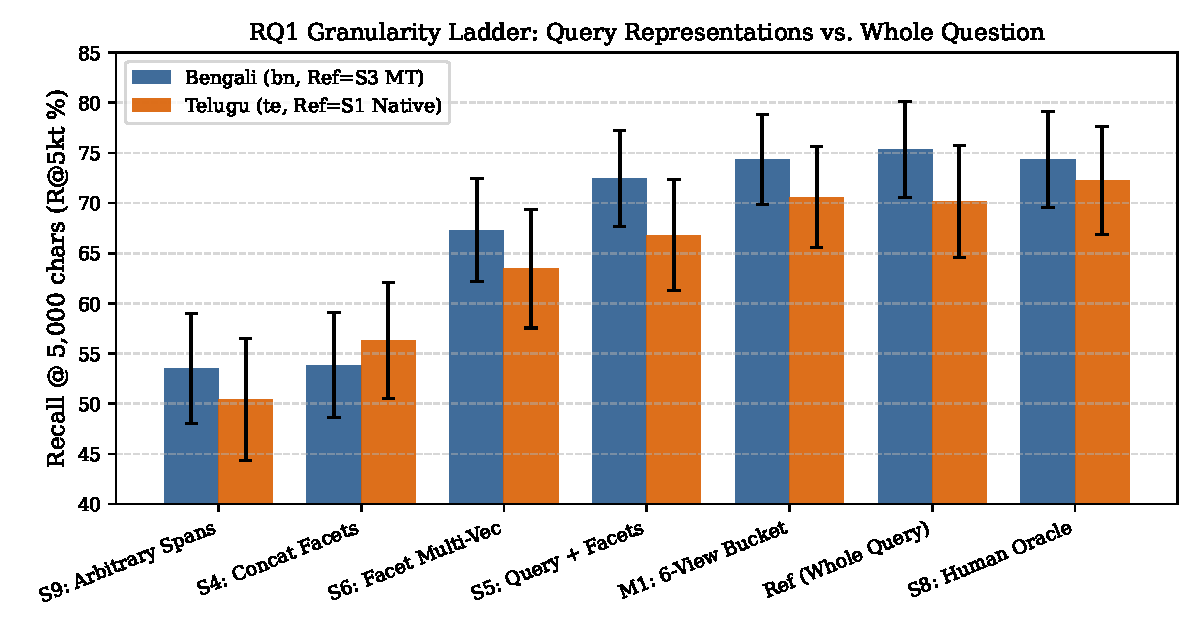
\includegraphics[width=0.88\linewidth]{fig1_granularity_ladder.pdf}
\caption{RQ1 Granularity Ladder: Recall at 5,000 characters (R@5kc) with 95\% bootstrap confidence intervals across query representations. The tested facet decomposition and fusion methods (S6, S9) underperform complete questions; we detected no improvement for semantic tag additions (S5) over matched random word additions (S5r).}
\label{fig:fig1_granularity_ladder}
\end{figure*}

As shown in Table~\ref{tab:granularity_table}, the tested facet decomposition and fusion methods underperform complete-query retrieval. On Bengali, S6 drops R@5kc from 75.32\% to 67.31\% ($-8.01$ pts, Holm-adjusted $p=0.015$). On Telugu, S6 drops R@5kc from 70.17\% to 63.45\% ($-6.72$ pts, Holm-adjusted $p=0.016$).

Crucially, our matched controls provide clear context on this performance gap:
\begin{enumerate}
    \item \textbf{Semantic vs.\ Arbitrary Slicing (S6 vs.\ S9):} Slicing the query into arbitrary contiguous 3-spans (S9) collapses further to 53.53\% (bn) and 50.42\% (te). While semantic facet grouping preserves more information than arbitrary slicing (+13.78 pts bn, +13.03 pts te), fragmenting query context damages representation quality in both conditions.
    \item \textbf{Content vs.\ Length Control (S5 vs.\ S5r):} Appending semantic facet tags to the whole question (S5: 72.44\% bn, 65.55\% te) yields no benefit over appending length-matched random dictionary words (S5r: 72.44\% bn, 67.23\% te; $p=1.0$ bn, $p=0.384$ te). We detected no improvement over the random-word control.
    \item \textbf{Ablation of Facet Components:} In post-hoc ablations, dropping the relation vector from S6 drops recall to 53.85\% (bn) and 47.90\% (te). Conversely, dropping entity vectors improves recall to 72.44\% (bn) and 68.49\% (te), indicating that dense encoders rely heavily on compositional predicate-argument relations rather than isolated entity tokens.
\end{enumerate}

\paragraph{Multi-View Sentence Buckets (M1) and Oracle Headroom.} Table~\ref{tab:m1_headroom} evaluates the individual views of M1, the tuned LSE ensemble, and an oracle view selector. Expanding the query into complete sentences preserves natural syntax: the LSE ensemble achieves 74.36\% (bn) and 70.59\% (te), statistically matching the single best whole question. An oracle selector demonstrates that meaningful headroom exists across diverse sentence perspectives (+2.56 pts bn, +5.04 pts te), though automated pooling does not fully capture this potential.

\begin{table}[t]
\centering
\small
\resizebox{\columnwidth}{!}{%
\begin{tabular}{lcc}
\toprule
\textbf{Query View / Configuration} & \textbf{Bengali (\texttt{bn})} & \textbf{Telugu (\texttt{te})} \\
\midrule
Primary Reference (S3 bn / S1 te) & 75.32\% & 70.17\% \\
View 1: Literal Translation        & 73.72\% & 70.17\% \\
View 2: Natural Translation        & 73.72\% & 70.59\% \\
View 3: English Paraphrase         & 72.44\% & 70.17\% \\
View 4: Declarative Cloze          & 74.04\% & 69.33\% \\
View 5: Native Paraphrase          & 68.59\% & 69.33\% \\
View 6: Romanized Script           & 28.85\% & 15.55\% \\
\midrule
\textbf{M1: LSE Ensemble} ($\beta=2.0$) & 74.36\% & 70.59\% \\
\textbf{ORACLE: 6-View Ceiling}   & \textbf{77.88\%} & \textbf{75.21\%} \\
\quad Headroom over Reference      & +2.56 pts ($p=.009$) & +5.04 pts ($p<.001$) \\
\bottomrule
\end{tabular}%
}
\caption{Evaluation of M1 sentence-level views, LSE ensemble, and oracle selector headroom (R@5kc).}
\label{tab:m1_headroom}
\end{table}

\subsection{RQ2: Translation Effects across Languages and Retrievers}
\label{sec:rq2_results}

Table~\ref{tab:encoder_table} evaluates the effect of machine translation across two multilingual encoders: BGE-M3 and multilingual-E5-small.

\begin{table}[t]
\centering
\small
\resizebox{\columnwidth}{!}{%
\begin{tabular}{llccc}
\toprule
\textbf{Track} & \textbf{Retriever} & \textbf{S1 (Native)} & \textbf{S3 (MT)} & \textbf{$\Delta$ (MT$-$Nat)} \\
\midrule
\multirow{2}{*}{Bengali (\texttt{bn})} & mE5-small (117M) & 61.54\% & 72.44\% & \textbf{+10.90 pts} \\
                                       & BGE-M3 (567M)    & 67.63\% & 75.32\% & \textbf{+7.69 pts} \\
\midrule
\multirow{2}{*}{Telugu (\texttt{te})}  & mE5-small (117M) & 61.34\% & 67.65\% & \textbf{+6.31 pts} \\
                                       & BGE-M3 (567M)    & 70.17\% & 69.33\% & \textbf{$-$0.84 pts} \\
\bottomrule
\end{tabular}%
}
\caption{RQ2: Effect of English translation across retrievers (R@5kc). Translation improves Bengali retrieval across both models, while native Telugu retrieval matches MT on BGE-M3.}
\label{tab:encoder_table}
\end{table}

As shown in Table~\ref{tab:encoder_table}:
\begin{itemize}
    \item For Bengali, translating queries into English provides substantial gains across both models: +10.90 pts on mE5-small ($61.54\% \to 72.44\%$) and +7.69 pts on BGE-M3 ($67.63\% \to 75.32\%$, Holm-adjusted $p < 0.001$).
    \item For Telugu, machine translation yields a +6.31 pt gain on mE5-small ($61.34\% \to 67.65\%$), but provides no measurable gain on BGE-M3, where native zero-shot retrieval performs comparably to translated queries ($70.17\%$ vs.\ $69.33\%$, $\Delta = -0.84$ pts, $p=1.0$).
\end{itemize}
Because BGE-M3 and mE5-small differ in parameter scale, pre-training data, and training objectives, we do not claim a general capacity scaling law; rather, these results demonstrate that the translation advantage is contingent on both the target language and the specific embedding retriever.

\subsection{RQ3: Channel Diversity and Candidate Budgets}
\label{sec:rq3_results}

Table~\ref{tab:channels_and_rerank} evaluates similarity channels under strictly matched candidate budgets, distinguishing pre-reranking candidate coverage from post-reranking character-budget performance.

\begin{table*}[t]
\centering
\small
\renewcommand{\arraystretch}{0.92}
\setlength{\tabcolsep}{4.5pt}
\resizebox{\textwidth}{!}{%
\begin{tabular}{lcccccc}
\toprule
\multirow{2}{*}{\textbf{Configuration / Pool Budget}} & \multicolumn{3}{c}{\textbf{Bengali (\texttt{bn}, $n=312$)}} & \multicolumn{3}{c}{\textbf{Telugu (\texttt{te}, $n=238$)}} \\
\cmidrule(lr){2-4} \cmidrule(lr){5-7}
 & \textbf{R@2kc} & \textbf{R@5kc} & \textbf{Candidate Coverage} & \textbf{R@2kc} & \textbf{R@5kc} & \textbf{Candidate Coverage} \\
\midrule
\multicolumn{7}{l}{\textit{First-Stage Retrieval (Fixed Budget: Top-100 Candidates)}} \\
Dense Single Channel (S3 bn / S1 te) & 62.82\% & 75.32\% & 85.90\% (R@100) & 57.98\% & 70.17\% & 83.61\% (R@100) \\
6-Channel RRF (Top-100 Candidates)   & 61.54\% & 75.00\% & 86.54\% (R@100) & 57.14\% & 69.33\% & 82.77\% (R@100) \\
\midrule
\multicolumn{7}{l}{\textit{First-Stage Retrieval (Fixed Budget: Top-200 Candidates)}} \\
Dense Single Channel (Top-200)       & 62.82\% & 75.32\% & 87.50\% (R@200) & 57.98\% & 70.17\% & 85.29\% (R@200) \\
6-Channel RRF (Top-200 Candidates)   & 61.54\% & 75.00\% & \textbf{88.46\%} (R@200) & 57.14\% & 69.33\% & \textbf{85.29\%} (R@200) \\
\midrule
\multicolumn{7}{l}{\textit{Cross-Encoder Reranked Retrieval (\texttt{bge-reranker-v2-m3})}} \\
R-Dense (Rerank Top-100 Dense)       & 66.67\% & \textbf{76.28\%} & 85.90\% (R@100) & \textbf{63.03\%} & \textbf{71.43\%} & 83.61\% (R@100) \\
R-Union100 (Rerank Top-100 6-Channel)& 66.03\% & 75.96\% & 86.54\% (R@100) & 62.61\% & 69.75\% & 82.77\% (R@100) \\
R-Union200 (Rerank Top-200 6-Channel)& \textbf{66.67\%} & 75.64\% & 86.86\% (R@100) & 62.18\% & 69.33\% & 85.29\% (R@100) \\
\bottomrule
\end{tabular}%
}
\caption{RQ3 Matched Evaluation: First-stage candidate coverage and cross-encoder reranking across strictly matched candidate budgets (top-100 vs.\ top-200). Under a matched top-100 budget, 6-channel RRF yields no gain over single-channel dense retrieval (86.54\% vs.\ 85.90\% bn; 82.77\% vs.\ 83.61\% te). Retaining top-200 candidates increases overall coverage, but cross-encoder reranking does not translate deep candidate gains into character-budget improvements.}
\label{tab:channels_and_rerank}
\end{table*}

As detailed in Table~\ref{tab:channels_and_rerank}:

\paragraph{Matched Candidate Budget Comparison.} When candidate budgets are strictly matched at top-100, 6-channel RRF achieves 86.54\% (bn) and 82.77\% (te) candidate recall, compared to 85.90\% (bn) and 83.61\% (te) for single-channel dense retrieval. Under this matched budget, multi-channel fusion yields a slight +0.64 pt shift on Bengali, but underperforms single-channel dense on Telugu ($-0.84$ pts). The coverage advantage from channel diversity only emerges when expanding candidate retention to top-200, reaching 88.46\% on Bengali (+0.96 pts over dense top-200) and matching dense top-200 on Telugu (85.29\%).

\paragraph{Post-Reranking Conversion under Character Budgets.} Applying \texttt{bge-reranker-v2-m3} over top-100 dense candidates (R-Dense) improves early precision, increasing R@2kc by +3.85 pts on Bengali ($62.82\% \to 66.67\%$) and +5.05 pts on Telugu ($57.98\% \to 63.03\%$). However, reranking the expanded top-200 hybrid pool (R-Union200) yields 75.64\% R@5kc on Bengali (vs.\ 76.28\% for R-Dense) and 69.33\% on Telugu (vs.\ 71.43\% for R-Dense). While deeper candidate pools capture additional relevant documents, the cross-encoder does not consistently promote these rescued candidates into top character cutoffs.

\section{Discussion and Limitations}
\label{sec:discussion}

\paragraph{Practical Engineering Implications.} (1)~\emph{Preserve Complete Query Context:} Explicitly splitting questions into entity, relation, and constraint keywords degrades dense retrieval. When expansion is desired, sentence-level paraphrases (M1) maintain compositional syntax much more effectively. (2)~\emph{Distinguish Generation from Ranking:} While multi-channel similarity ensembles can increase candidate pool recall, downstream cross-encoders require careful alignment to rank diverse multi-channel evidence ahead of lexical distractors.

\paragraph{Limitations.} (1)~\emph{Relevance Metric:} XOR-TyDi evaluates relevance via short answer substring containment, which may introduce noise when target strings occur in non-relevant contexts. (2)~\emph{Candidate Pooling Protocol:} Because exhaustive 21M dense cross-attention across dozens of query variants is computationally prohibitive, evaluations operate over a pooled candidate corpus (ceilings 86--91\%). (3)~\emph{Language Scope:} Experiments focus on Bengali and Telugu; broader language typologies remain open for future work.

\section{Conclusion}
\label{sec:conclusion}

On XOR-TyDi Bengali- and Telugu-to-English retrieval, the tested facet decomposition and fusion methods underperformed complete-query retrieval, and we detected no improvement from semantic expansion over a matched random-word control. Translation effects differed markedly across languages and encoders: Bengali benefited consistently from machine translation, whereas native Telugu queries matched translation on BGE-M3. Under matched candidate budgets, multi-channel similarity fusion only surfaced additional candidates when candidate retention was expanded to top-200, and cross-encoder reranking did not convert these deeper candidates into character-budget gains. These results caution against assuming that explicit query decomposition repairs cross-lingual representation loss and motivate evaluating candidate generation under matched budgets separately from final ranking.

\bibliography{custom}

\begin{table*}[t]
\centering
\small
\resizebox{\textwidth}{!}{%
\begin{tabular}{lll}
\toprule
\textbf{System ID} & \textbf{Family} & \textbf{Operational Definition} \\
\midrule
\textbf{S1} & Dense Baseline & Native query encoded directly with BGE-M3 zero-shot bi-encoder. \\
\textbf{S2} & Sparse Baseline & BM25 lexical matching over 21M Lucene index using machine-translated English query. \\
\textbf{S3} & Dense MT Reference & Machine-translated English query encoded directly with BGE-M3 (Bengali Reference). \\
\textbf{S8} & Human Reference Translation & Human English reference translation from XOR-TyDi evaluated strictly as a diagnostic reference. \\
\midrule
\textbf{S4} & Structured Baseline & Extracted semantic entity and constraint facets concatenated into a single string. \\
\textbf{S5} & Structured Expansion & Original question concatenated with structured entity and constraint tags. \\
\textbf{S5r} & Matched Length Control & Original question concatenated with length-matched random dictionary words. \\
\textbf{S6} & Multi-Vector Facets & Semantic facets (entity, relation, constraints) encoded independently and fused via normalized scores. \\
\textbf{S9} & Arbitrary Span Control & Original question sliced into three arbitrary contiguous token spans; scored via S6 fusion formula. \\
\midrule
\textbf{M1} & Sentence Buckets & 6 full-sentence multi-view paraphrases aggregated via Log-Sum-Exp soft-max pooling. \\
\textbf{6-Channel RRF} & Channel Fusion & Reciprocal Rank Fusion ($k=60$) over Dense, Sparse, and ColBERT MaxSim (native + MT). \\
\textbf{R-Dense} & Reranked Baseline & Cross-encoder (\texttt{bge-reranker-v2-m3}) applied over top-100 dense candidate pool. \\
\textbf{R-Union200} & Reranked Fusion & Cross-encoder applied over top-200 6-channel candidate pool. \\
\bottomrule
\end{tabular}%
}
\caption{Taxonomy and operational definitions of evaluated systems and matched controls.}
\label{tab:system_taxonomy}
\end{table*}

\begin{table*}[t]
\centering
\small
\resizebox{\textwidth}{!}{%
\begin{tabular}{p{3.5cm}p{13cm}}
\toprule
\textbf{Task} & \textbf{Prompt Instruction and Output Schema} \\
\midrule
\textbf{Machine Translation} & Translate the following Indic question into fluent, grammatically natural English for document retrieval. Return strictly JSON: \texttt{\{"translation": "..."\}}. \\
\midrule
\textbf{Semantic Facet Decomposition (S6)} & Decompose the following question into structured search facets. Extract: (1) \texttt{entities}: named entities or core nouns; (2) \texttt{relation}: the central predicate or verb phrase; (3) \texttt{constraints}: temporal, geographical, or numerical qualifiers. Return strictly JSON matching the specified schema. \\
\midrule
\textbf{Multi-View Paraphrases (M1)} & Generate 6 diverse sentence-level views of the input question: (1) literal translation, (2) natural fluent translation, (3) English paraphrase, (4) native source paraphrase, (5) declarative cloze query, and (6) romanized transliteration. Return strictly JSON: \texttt{\{"views": ["...", ..., "..."]\}}. \\
\bottomrule
\end{tabular}%
}
\caption{System prompt instructions used for automated query transformations.}
\label{tab:prompt_templates}
\end{table*}

\newpage
\appendix

\section{System Taxonomy and Operational Definitions}
\label{sec:appendix_taxonomy}

Table~\ref{tab:system_taxonomy} outlines the operational definitions of evaluated retrieval systems and matched controls.

\section{Prompt Templates for LLM Transformations}
\label{sec:appendix_prompts}

Table~\ref{tab:prompt_templates} details the prompt instructions used for query translation, semantic facet decomposition, and full-sentence multi-view generation.

\end{document}
